\documentclass[14pt]{extbook}
\usepackage{multicol, enumerate, enumitem, hyperref, color, soul, setspace, parskip, fancyhdr} %General Packages
\usepackage{amssymb, amsthm, amsmath, latexsym, units, mathtools} %Math Packages
\everymath{\displaystyle} %All math in Display Style
% Packages with additional options
\usepackage[headsep=0.5cm,headheight=12pt, left=1 in,right= 1 in,top= 1 in,bottom= 1 in]{geometry}
\usepackage[usenames,dvipsnames]{xcolor}
\usepackage{dashrule}  % Package to use the command below to create lines between items
\newcommand{\litem}[1]{\item#1\hspace*{-1cm}\rule{\textwidth}{0.4pt}}
\pagestyle{fancy}
\lhead{Progress Quiz 6}
\chead{}
\rhead{Version B}
\lfoot{9689-6866}
\cfoot{}
\rfoot{Spring 2021}
\begin{document}

\begin{enumerate}
\litem{
Graph the equation below.\[ f(x) = -(x-4)^2 - 20 \]\begin{enumerate}[label=\Alph*.]
\begin{multicols}{2}\item 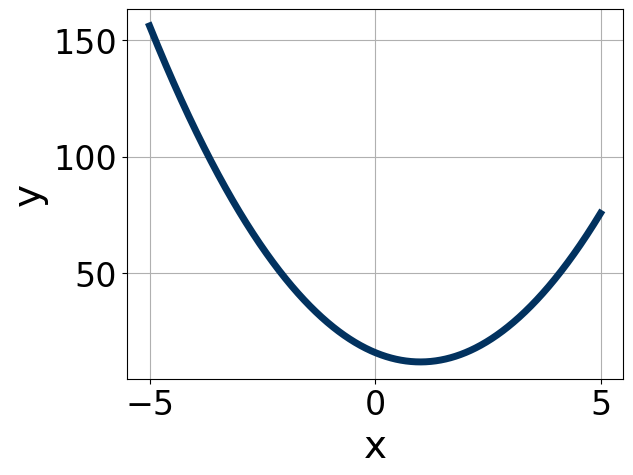
\includegraphics[width = 0.3\textwidth]{../Figures/quadraticEquationToGraphAB.png}\item 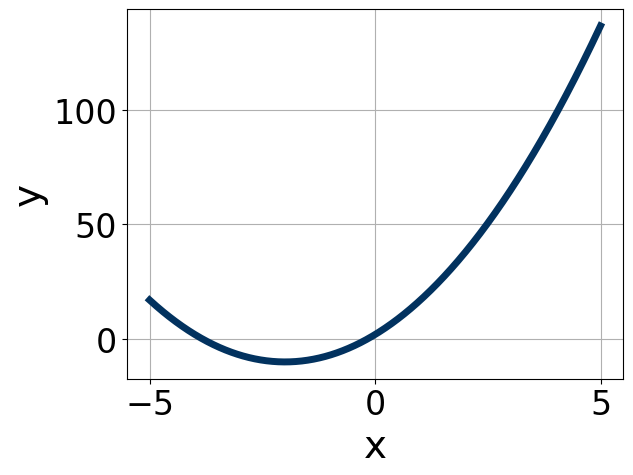
\includegraphics[width = 0.3\textwidth]{../Figures/quadraticEquationToGraphBB.png}\item 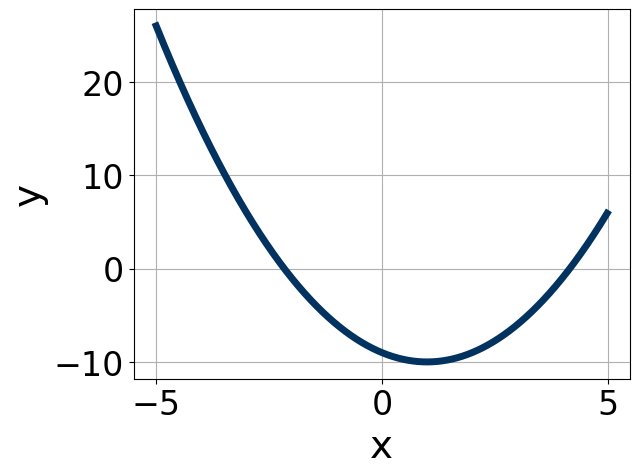
\includegraphics[width = 0.3\textwidth]{../Figures/quadraticEquationToGraphCB.png}\item 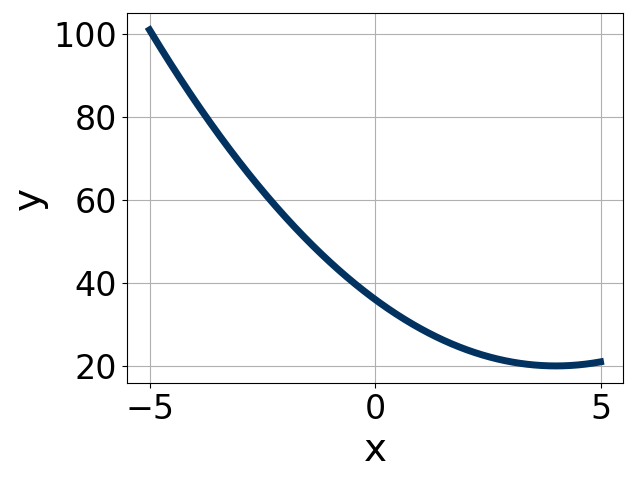
\includegraphics[width = 0.3\textwidth]{../Figures/quadraticEquationToGraphDB.png}\end{multicols}\item None of the above.
\end{enumerate} }
\litem{
Solve the quadratic equation below. Then, choose the intervals that the solutions belong to, with $x_1 \leq x_2$ (if they exist).\[ -10x^{2} -15 x + 4 = 0 \]\begin{enumerate}[label=\Alph*.]
\item \( x_1 \in [-2.44, -1.81] \text{ and } x_2 \in [16.5, 17.7] \)
\item \( x_1 \in [-0.73, -0.16] \text{ and } x_2 \in [0.5, 1.8] \)
\item \( x_1 \in [-20.62, -20.05] \text{ and } x_2 \in [18.7, 20.4] \)
\item \( x_1 \in [-1.97, -0.9] \text{ and } x_2 \in [-0.1, 0.8] \)
\item \( \text{There are no Real solutions.} \)

\end{enumerate} }
\litem{
Solve the quadratic equation below. Then, choose the intervals that the solutions $x_1$ and $x_2$ belong to, with $x_1 \leq x_2$.\[ 10x^{2} -57 x + 54 = 0 \]\begin{enumerate}[label=\Alph*.]
\item \( x_1 \in [1.02, 1.24] \text{ and } x_2 \in [2.99, 5.27] \)
\item \( x_1 \in [11.89, 12.18] \text{ and } x_2 \in [44.58, 45.71] \)
\item \( x_1 \in [0.3, 0.68] \text{ and } x_2 \in [13.03, 15.79] \)
\item \( x_1 \in [0.73, 1.14] \text{ and } x_2 \in [5.86, 6.19] \)
\item \( x_1 \in [2.24, 2.32] \text{ and } x_2 \in [1.89, 2.67] \)

\end{enumerate} }
\litem{
Write the equation of the graph presented below in the form $f(x)=ax^2+bx+c$, assuming  $a=1$ or $a=-1$. Then, choose the intervals that $a, b,$ and $c$ belong to.
\begin{center}
    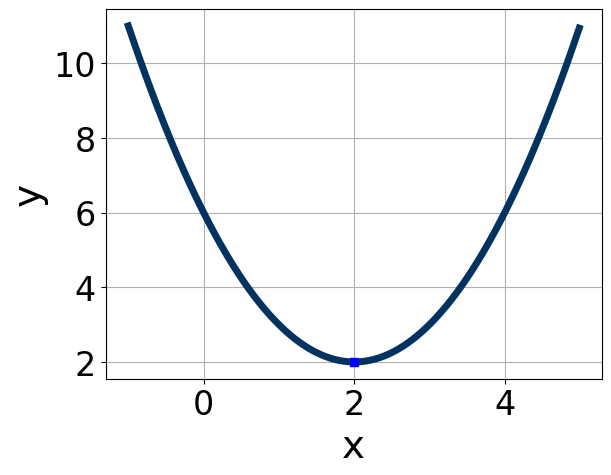
\includegraphics[width=0.5\textwidth]{../Figures/quadraticGraphToEquationCopyB.png}
\end{center}
\begin{enumerate}[label=\Alph*.]
\item \( a \in [-4, 0], \hspace*{5mm} b \in [2, 5], \text{ and } \hspace*{5mm} c \in [2, 5] \)
\item \( a \in [-4, 0], \hspace*{5mm} b \in [2, 5], \text{ and } \hspace*{5mm} c \in [-17, -9] \)
\item \( a \in [0, 5], \hspace*{5mm} b \in [2, 5], \text{ and } \hspace*{5mm} c \in [-6, -2] \)
\item \( a \in [-4, 0], \hspace*{5mm} b \in [-5, 0], \text{ and } \hspace*{5mm} c \in [-17, -9] \)
\item \( a \in [0, 5], \hspace*{5mm} b \in [-5, 0], \text{ and } \hspace*{5mm} c \in [-6, -2] \)

\end{enumerate} }
\litem{
Factor the quadratic below. Then, choose the intervals that contain the constants in the form $(ax+b)(cx+d); b \leq d.$\[ 24x^{2} +50 x + 25 \]\begin{enumerate}[label=\Alph*.]
\item \( a \in [1.93, 3.39], \hspace*{5mm} b \in [5, 8], \hspace*{5mm} c \in [7.77, 8.04], \text{ and } \hspace*{5mm} d \in [0, 7] \)
\item \( a \in [5.77, 7.19], \hspace*{5mm} b \in [5, 8], \hspace*{5mm} c \in [3.98, 4.48], \text{ and } \hspace*{5mm} d \in [0, 7] \)
\item \( a \in [10.85, 12.25], \hspace*{5mm} b \in [5, 8], \hspace*{5mm} c \in [1.48, 2.94], \text{ and } \hspace*{5mm} d \in [0, 7] \)
\item \( a \in [-0.37, 1.35], \hspace*{5mm} b \in [16, 30], \hspace*{5mm} c \in [0.52, 1.28], \text{ and } \hspace*{5mm} d \in [30, 32] \)
\item \( \text{None of the above.} \)

\end{enumerate} }
\litem{
Write the equation of the graph presented below in the form $f(x)=ax^2+bx+c$, assuming  $a=1$ or $a=-1$. Then, choose the intervals that $a, b,$ and $c$ belong to.
\begin{center}
    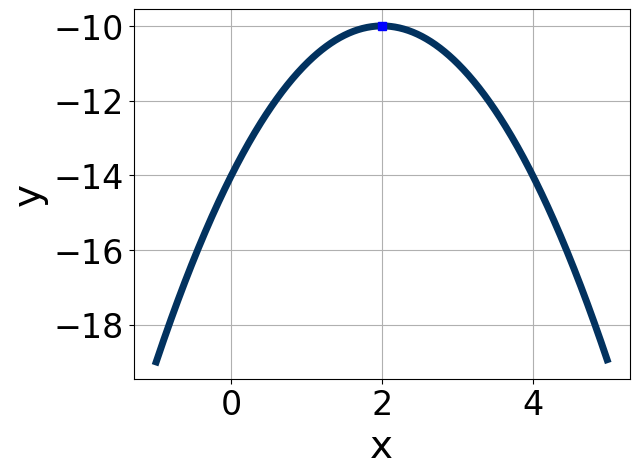
\includegraphics[width=0.5\textwidth]{../Figures/quadraticGraphToEquationB.png}
\end{center}
\begin{enumerate}[label=\Alph*.]
\item \( a \in [-1, 0], \hspace*{5mm} b \in [0, 5], \text{ and } \hspace*{5mm} c \in [-15, -10] \)
\item \( a \in [0, 3], \hspace*{5mm} b \in [-5, -2], \text{ and } \hspace*{5mm} c \in [-5, -1] \)
\item \( a \in [-1, 0], \hspace*{5mm} b \in [-5, -2], \text{ and } \hspace*{5mm} c \in [-15, -10] \)
\item \( a \in [0, 3], \hspace*{5mm} b \in [0, 5], \text{ and } \hspace*{5mm} c \in [-5, -1] \)
\item \( a \in [0, 3], \hspace*{5mm} b \in [0, 5], \text{ and } \hspace*{5mm} c \in [10, 13] \)

\end{enumerate} }
\litem{
Solve the quadratic equation below. Then, choose the intervals that the solutions $x_1$ and $x_2$ belong to, with $x_1 \leq x_2$.\[ 25x^{2} -60 x + 36 = 0 \]\begin{enumerate}[label=\Alph*.]
\item \( x_1 \in [0.11, 0.38] \text{ and } x_2 \in [5.32, 6.2] \)
\item \( x_1 \in [0.37, 0.4] \text{ and } x_2 \in [3.14, 4.16] \)
\item \( x_1 \in [0.54, 0.62] \text{ and } x_2 \in [1.85, 3.34] \)
\item \( x_1 \in [29.79, 30.05] \text{ and } x_2 \in [28.61, 30.86] \)
\item \( x_1 \in [1.06, 1.27] \text{ and } x_2 \in [-0.39, 1.21] \)

\end{enumerate} }
\litem{
Factor the quadratic below. Then, choose the intervals that contain the constants in the form $(ax+b)(cx+d); b \leq d.$\[ 54x^{2} +75 x + 25 \]\begin{enumerate}[label=\Alph*.]
\item \( a \in [2.5, 5.6], \hspace*{5mm} b \in [-1, 11], \hspace*{5mm} c \in [17.48, 18.73], \text{ and } \hspace*{5mm} d \in [3, 6] \)
\item \( a \in [25.6, 27.6], \hspace*{5mm} b \in [-1, 11], \hspace*{5mm} c \in [1.6, 2.26], \text{ and } \hspace*{5mm} d \in [3, 6] \)
\item \( a \in [-2.5, 2.9], \hspace*{5mm} b \in [29, 34], \hspace*{5mm} c \in [0.58, 1.26], \text{ and } \hspace*{5mm} d \in [44, 47] \)
\item \( a \in [6, 9.5], \hspace*{5mm} b \in [-1, 11], \hspace*{5mm} c \in [5.79, 7.66], \text{ and } \hspace*{5mm} d \in [3, 6] \)
\item \( \text{None of the above.} \)

\end{enumerate} }
\litem{
Solve the quadratic equation below. Then, choose the intervals that the solutions belong to, with $x_1 \leq x_2$ (if they exist).\[ -16x^{2} -8 x + 7 = 0 \]\begin{enumerate}[label=\Alph*.]
\item \( x_1 \in [-3.2, -0.6] \text{ and } x_2 \in [0.3, 0.64] \)
\item \( x_1 \in [-23.2, -22] \text{ and } x_2 \in [22.14, 23.22] \)
\item \( x_1 \in [-0.5, 1.4] \text{ and } x_2 \in [0.9, 1.34] \)
\item \( x_1 \in [-7.5, -6.5] \text{ and } x_2 \in [14.53, 15.65] \)
\item \( \text{There are no Real solutions.} \)

\end{enumerate} }
\litem{
Graph the equation below.\[ f(x) = -(x+3)^2 - 10 \]\begin{enumerate}[label=\Alph*.]
\begin{multicols}{2}\item 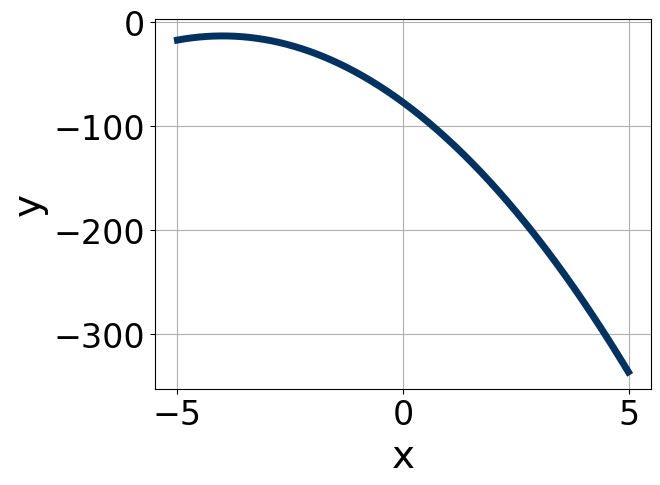
\includegraphics[width = 0.3\textwidth]{../Figures/quadraticEquationToGraphCopyAB.png}\item 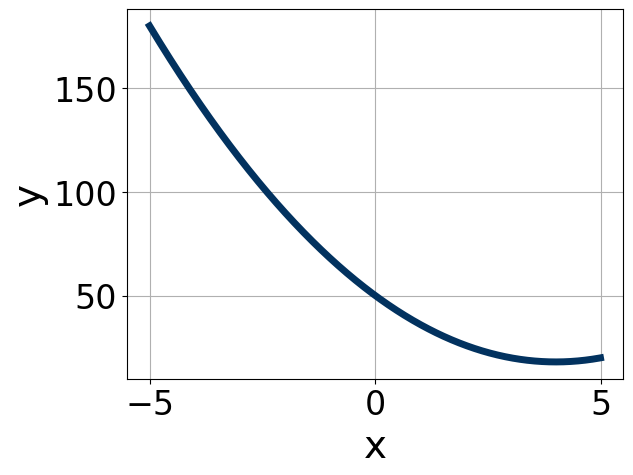
\includegraphics[width = 0.3\textwidth]{../Figures/quadraticEquationToGraphCopyBB.png}\item 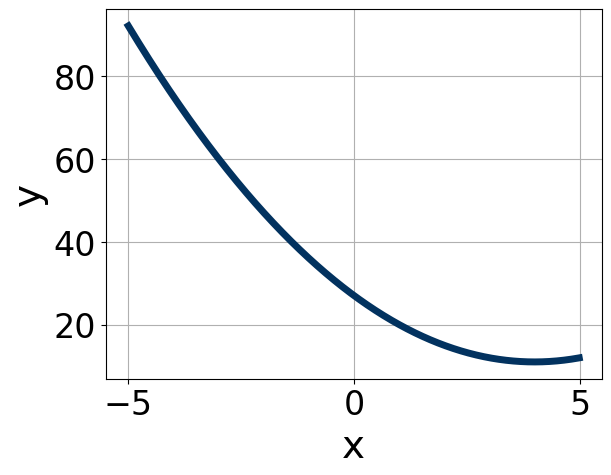
\includegraphics[width = 0.3\textwidth]{../Figures/quadraticEquationToGraphCopyCB.png}\item 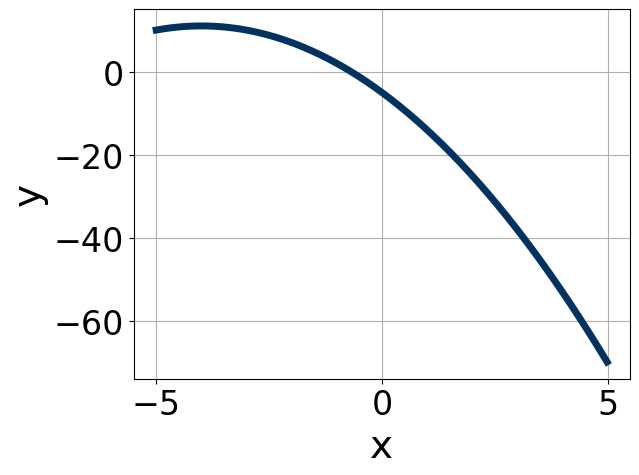
\includegraphics[width = 0.3\textwidth]{../Figures/quadraticEquationToGraphCopyDB.png}\end{multicols}\item None of the above.
\end{enumerate} }
\end{enumerate}

\end{document}